\chapter{Implementation}

The design for the prototype I and prototype II detailed in the chapter \ref{DA} were implemented through iterative development process where the design for prototype I was drafted and implemented first, followed by the prototype II. This chapter details the procedure which was followed during the development and implementation of the thesis.  

\section{Native Cuttlefish Application} 
The native cuttlefish application is a 64-bit windows application, developed in C++ language using the Microsoft Visual Studio 12 SDK and the compiler used to build the code is Microsoft C/C++ V120 compiler. A project could be compiled either as static library or an executable in release or debug mode. The input for the application i.e. the path of the main configuration file, is presented as command line argument. The output generated by the application depends on the type of output component chosen in the component configuration. For each component, the behavior of the component is logged in the performance report and a log file for overall pipeline is written to the working directory at the end of the execution. This helps to analyze the component performance as well as to know the possible error by looking into the pipeline execution trace in case of a failure. Some of the projects of the application use external libraries (like zlib, little cms , poly2tri, boost, itk etc) which are either used as headers only or compiled for windows platform and linked as static library. 

Some parts of the computation performed by the application is on the GPU (graphics processing unit) and the code performing this computation is written and compiled using CUDA Toolkit. Another library used by the application is OpenGL(Open Graphics Library) wherein various powerful visualization features of the library are used for rendering, texture mapping etc. The minimum OpenGL version that is needed by the application to run should be 2.0 as one of the APIs used- glCreateProgram, is available only in version 2.0 or higher. The native application has a strong dependency on availability of graphics library and CUDA.     

\section{Prerequisites for Distributed Cuttlefish Application Development} 

The goal of the thesis was earlier to provide a cloud service which could take the input from the user and do the computation using the cloud instances and provide the bitmaps as the output. With this goal, the native application had to be modified such that it could run on the cloud instances provided by the AWS (Amazon Web Services) as PAAS (Platform as a Service). The cluster of instances which formed the {\lq}cloud{\rq} were the basic Amazon EC2 instances which were virtual machines with Linux operating system. As the basic instances were virtual machines which were not GPU accelerated i.e. they did not have access to a GPU, and therefore the code which performed the GPU computing had to be changed such that only when the GPU is available, the code is compiled and used . So, this change to the native application code was done by creating a new configuration, other than release and debug, called as the CUDA\_FREE\_CONFIG which got rid of the dependency on availability of CUDA on the system running the application. The code performing the GPU computing is defined under if-defs to get the CUDA\_FREE\_CONFIG as seen in the Listing \ref{lst:CFC}

\begin{lstlisting}[language=C++,label={lst:CFC},caption={CUDA free configuration}]
//....
#ifndef CUDA_FREE	
			inline operator std::shared_ptr<VoxelSliceGPU>()
			{
				if (m_channel == m_invalidIndex)
					return nullptr;
				validate();
				return std::dynamic_pointer_cast<VoxelSliceGPU>(m_pContainer->m_slices[m_channel][m_slice]);
			}

#endif
//....
\end{lstlisting}

The CUDA\_FREE\_CONFIG configuration was still only for windows platform and the projects needed to be compiled such that they were compatible with Linux and it was necessary to get rid of the windows specific dependencies. To achieve portability and make the cross-platform build of the application possible, a configuration file called as the {\lq}CMakeLists.txt{\rq}  was written for each project of the application. Using CMake, an open-source system that manages the build process for an operating system in a compiler independent manner, all the project's cmakelists.txt files were parsed to generate the desired solution (depending on the generator chosen by the developer) i.e. the solution file could be Microsoft Visual Studio 12 solution or Unix makefiles or Eclipse CDT Unix makefiles. After using cmake to generate makefiles for linux system, the process to remove the windows specific code was started but could not be completed  due to time limitation (as it required rigorous amount changes). Hence, instead of using basic EC2 instances running Linux, a decision to use basic EC2 instances running windows operating system was made.    

The next step was to check if the CUDA free application configuration could run on an instance i.e. virtual machine with windows operating system. The application crashed in the call to the glCreateProgram api on the instance as the OpenGL version was 1.1. The fix for this issue would be to make OpenGL version 2.0 available on the instance i.e. the Virtual Machine. This cannot be done as OpenGL has a hardware limitation and the virtual machines use virtual GPUs which cannot support OpenGL 2.0 and provide support for only GPU basics. Hence, as most of the basic cloud instances (irrespective of the vendor/provider) are virtual machines supporting only GPU basics, the application could not be run on these instances. Therefore, instead of using a cloud of virtual machines as compute nodes, a decision to use physical processors as compute nodes was made, hence instead of cloud computing, cluster computing was chosen as the distributed system . 

The physical processors are 64-bit machines which run windows operating system and have access to the GPUs with the OpenGL 2.0 version available to the application. These physical machines are connected via the enterprise network. Though the compute nodes already had a common network, to use them as a cluster there was a need to perform a few installations to enable `clustering` as detailed in the section \ref{ICS}. 


\section{Installation and Cluster Set-up} \label{ICS}

To begin with, a cluster with 2 nodes was created such that the nodes were connected to each other via a common network. To check if the cluster nodes could communicate, a simple ping test was performed. The next step was to write a program which performed a simple task in a distributed fashion and to run it on the cluster. For the cluster to work as system where the processing can be shared, there needs to be a way in which the cluster nodes can be named and the work to be done by each node could be distinguished i.e. assign roles to the nodes. There are many types of hardware/software solutions for the cluster which enable naming and role distinction among cluster nodes. The decision to use MPI-Message Passing Interface, was made to achieve naming and role assignment amongst the cluster nodes. MPI is the open standard specification for message passing libraries which provide apis to enable communication, role distinction and naming amongst the cluster nodes. There are various implementations of the specification available which basically perform the same thing i.e. message passing amongst the cluster nodes but are different with respect to the platform they support, commands to compile and launch the program, debugging and developed by different institutions. 
Some of the implementations are free-ware and some aren\textquotesingle t. As currently, cuttlefish is a windows application developed using Microsoft visual studio, the Microsoft\textquotesingle s implementation of MPI called as MSMPI is used. 

To use MSMPI, on each node of the cluster, the MS-MPI SDK is downloaded and installed. To verify if the installation and setup is done correctly, the environment variables are checked using the command {\lq} set MSMPI {\rq}. The environment variables which are particularly interesting are \$MSMPI\_INC\$, \$MSMPI\_BIN\$, and \$MSMPI\_LIB64\$. The table \ref{MSMPI-ENV} summarizes the details about these variable. 

\begin{table}[]
\centering
\label{my-label}
\begin{tabular}{|l|l|l|ll}
\cline{1-3}
\begin{tabular}[c]{@{}l@{}}Environment\\ Variable\end{tabular} & Value                                       & Significance                                 &  &  \\ \cline{1-3}
MSMPI\_INC                                                     & ..\textbackslash Microsoft SDKs\textbackslash MPI\textbackslash Include               & Path to find the headers                     &  &  \\ \cline{1-3}
MSMPI\_LIB64                                                   & ..\textbackslash Microsoft SDKs\textbackslash MPI\textbackslash Lib\textbackslash x64\textbackslash & Path to find the libraries for 64 bit system &  &  \\ \cline{1-3}
MSMPI\_BIN                                                     & ..\textbackslash Microsoft MPI\textbackslash Bin\textbackslash          & Path to find the binaries                    &  &  \\ \cline{1-3}
\end{tabular}
\label{MSMPI-ENV}
\caption{ MS-MPI Environment Variable}
\end{table}

To compile a program which is designed to run on the cluster where the nodes communicate using MPI, the directories which help to resolve the reference to header files specific to MPI and path to the libraries which resolve linking to the MPI functions are incorporated in the project. Before running the program, a process management system which allows to manage the parallel processes on the cluster nodes should be executed on each of the cluster node. For MPI, the process management system used is called as SMPD (Simple Multipurpose Daemon) which is part of the software component of the process manager provided by Intel. It allows starting and managing parallel jobs on the cluster nodes. SMPD is used as a windows service and is set during the MPI installation. Ideally, the version of SMPD running on each node in the cluster should be same, although if there are different versions of SMPD, there is a possibility to disable the check for the versions. As the SMPD service is set during MPI installation, the version of SMPD is compatible with the mpiexec version. To run the program, mpiexec command is used with the arguments specifying the number of hosts, host names, the directory where the executable for application to be launched is available, the name of the executable followed by arguments to the executable. The listing \ref{lst:MPIC} is an example of the command syntax to launch the application using mpiexec command.  

\begin{lstlisting}[language=C++,label={lst:MPIC},caption={mpiexec syntax}]
mpiexec -hosts 2 PC2215 PC2286 -wdir \\pc2215\bin\Release\ Cuttlefish.exe \\pc2215\mainconf.json
\end{lstlisting}  
	
\section{Introduction to New Components}

After the set-up and installation, the next step was the implementation of the prototype I followed by the implementation of prototype II. The components of both the prototypes are discussed in detail in the chapter \ref{DA}. Each of the new component is inherited from the class called as the \textit{PrintingComponent} and is registered using the component name. During the creation of the pipeline i.e. when the component configuration is parsed, each of the component is created and initialized with the required parameter values. The parameter values for each component are set in the configuration file. The Figure \ref{fig:Componentdiagram} summarizes the new components(underlined component names) introduced during the implementation of the thesis.

\begin{figure}[ht!]
\centering
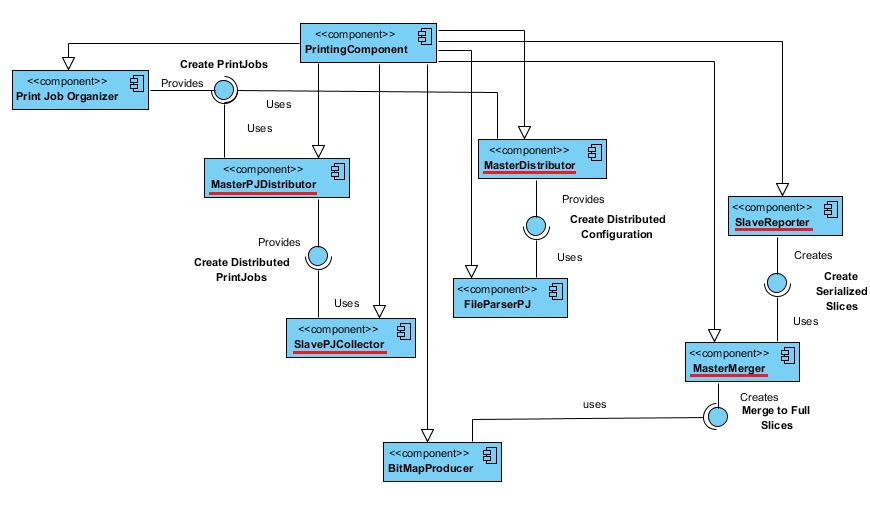
\includegraphics[scale=0.8]{Componentdiagram.PNG}
\caption{Component Diagram For New Components}
\label{fig:Componentdiagram}
\end{figure}

Each component has an input it receives from another component and an output that it generates which may be used by the following component in the pipeline(if any). The dependency is depicted in the Figure \ref{fig:Componentdiagram} by the {\lq}lollipop{\rq} symbol where in the half circle depicts interface exported by the component and the circle represents the interface that is imported by the component, for example, the component \textit{MasterDistributorPJ} uses the print job created by the \textit{PrintJobOrganizer} and provides the print jobs with distributed print objects used by the \textit{SlavePJCollector}.

\subsection{Introduction to the New Classes}
The new classes which were implemented during the thesis are enlisted in the Table \ref{CSPI} for prototype I, in the Table \ref{CSPII} for prototype II and common classes used by both the prototypes are listed in Table \ref{ComClass}. 

\begin{table}[ht]
\centering
\caption{Class specific for Prototype I}
\label{CSPI}
\begin{tabular}{|l|l|l}
\cline{1-2}
\textbf{Class}              & 
\textbf{Purpose}                                                                                                                                                                                                &  \\ \cline{1-2}
MasterDistributor & \begin{tabular}[c]{@{}l@{}}Class for slave work item creation and distribution. \\ The work item created is the main configuration file \\ containing the assigned number of print object files.\end{tabular} &  \\ \cline{1-2}
\end{tabular}
\end{table}

\begin{table}[ht]
\centering
\caption{Classes specific for Prototype II}
\label{CSPII}
\begin{tabular}{|l|l|l}
\cline{1-2}
\textbf{Class}      & \textbf{Purpose}                                                                                                                                                                   &  \\ \cline{1-2}
MasterPJDistributor & \begin{tabular}[c]{@{}l@{}}Class for creation of print jobs with the print objects \\ distributed using the cost function and \\ serialization of the print jobs\end{tabular}      &  \\ \cline{1-2}
SlavePJCollector    & \begin{tabular}[c]{@{}l@{}}Class for collection of the serialized print job, \\ de-serialization of the print jobs and loading\\ the texture data to the node memory.\end{tabular} &  \\ \cline{1-2}
\end{tabular}
\end{table}

\begin{table}[ht]
\centering
\caption{Common Classes For Prototype I and II}
\label{ComClass}
\begin{tabular}{|l|l|l}
\cline{1-2}
\textbf{Class}                & \textbf{Purpose}                                                                                                                                                           &  \\ \cline{1-2}
MasterPrintingSoftware        & Creates and manages the printing software for the master node                                                                                                              &  \\ \cline{1-2}
SlavePrintingSoftware         & Creates and manages the printing software for the slave node                                                                                                               &  \\ \cline{1-2}
P3DNetworkComm                & Interface exposing the methods for communication                                                                                                                           &  \\ \cline{1-2}
P3dNetworkCommMPI             & \begin{tabular}[c]{@{}l@{}}Implements the interface methods using MPI as \\ the message passing library\end{tabular}                                                       &  \\ \cline{1-2}
DistributedComponentParser    & Parser for the JSON files used for distributed computing                                                                                                                   &  \\ \cline{1-2}
DistributedComponentInitiator & \begin{tabular}[c]{@{}l@{}}Initiator class for distributed computing. It manages \\ the cluster creation, execution and shut down of the\\ printing software\end{tabular}  &  \\ \cline{1-2}
SyncVoxelSlicesContainer      & \begin{tabular}[c]{@{}l@{}}Synchronized voxel slice container allowing \\ synchronous access to multiple threads\end{tabular}                                              &  \\ \cline{1-2}
MasterMergerWorker            & \begin{tabular}[c]{@{}l@{}}Interface exposing methods for performing \\ collection of metadata, de-serialization and\\  writing partial slices to full slices\end{tabular} &  \\ \cline{1-2}
MasterMergerWorkerImpl        & \begin{tabular}[c]{@{}l@{}}Implementation of the MasterMergerWorker class \\ with a thread per slave\end{tabular}                                                          &  \\ \cline{1-2}
DistributedCostFunction       & \begin{tabular}[c]{@{}l@{}}Class for calculation of the threshold and cost \\ function used for load distribution\end{tabular}                                             &  \\ \cline{1-2}
SlaveReporter                 & \begin{tabular}[c]{@{}l@{}}Class which performs serialization of the slices \\ and reports them to master\end{tabular}                                                     &  \\ \cline{1-2}
MasterMerger                  & \begin{tabular}[c]{@{}l@{}}Class performing collection of partial slices \\ and generation of merged full slices\end{tabular}                                              &  \\ \cline{1-2}
SlaveDataBuffer               & Synchronous queue used by the thread of slave reporter class                                                                                                               &  \\ \cline{1-2}
\end{tabular}
\end{table}

\begin{table}[ht]
\centering
\caption{Projects for Distributed Computing}
\label{ProDC}
\begin{tabular}{|l|l|l|ll}
\cline{1-3}
Project                  & Components / Classes                                                                                                              & Properties                                                                                                                                                                                                                                                                                                                   &  &  \\ \cline{1-3}
P3DDistributedCuttlefish & \begin{tabular}[c]{@{}l@{}}MasterMerger\\ MasterDistributor\\ MasterPJDistributor\\ SlaveReporter\\ SlavePJCollector\end{tabular} & \begin{tabular}[c]{@{}l@{}}1.Project contains the components which are \\ implemented for distributed computing. \\ 2.The project is built as a dynamic linking library. \\ 3.The project uses the Zlib, rapidjson external libraries.\end{tabular}                                                                      &  &  \\ \cline{1-3}
P3DDistributedUtility    & \begin{tabular}[c]{@{}l@{}}MasterPrintingSoftware\\ SlavePrintingSoftware\\ DistributedComputingInitiator\end{tabular}            & \begin{tabular}[c]{@{}l@{}}1. Project contains the classes implementing the \\ printing software and the initiator class for\\ distributed computing\\ 2.The project is built as a static library. \\ 3.The project uses rapidjson external library.\end{tabular}                                                     &  &  \\ \cline{1-3}
P3DNetworkComm           & \begin{tabular}[c]{@{}l@{}}P3DNetComm\\ P3DNetCommMPI\end{tabular}                                                                & \begin{tabular}[c]{@{}l@{}}1.Project contains the interface exporting the \\ methods used for communication over the network \\ and an MPI specific implementation of the interface. \\ 2.The project is built as a dynamic linking library\\ 3.MS-MPI library is the external library used \\ in the project.\end{tabular} &  &  \\ \cline{1-3}
\end{tabular}
\end{table}


\subsection{Code Organization}

The solution for the application is generated using the CMAKE tool with each project having it's own CMakeLists.txt file. The CMakeLists.txt file specifies the properties of the project such as the project would be built as an executable or static library or dynamic library, the libraries it needs to linked to, the include directories etc. Through the thesis, the code written is organized in 3 different projects namely P3DDistributedCuttlefish, P3DDistributedUtility and P3DNetworkComm. The Table \ref{ProDC} describes code organization in the projects named. Some of the directives of CMake which influence the generator output of a project are add\_library, add\_subdirectory, target\_link\_library  and add\_dependencies. The Table \ref{CDirec} details the directive used.

\begin{table}[]
\centering
\caption{Cmake Directives}
\label{CDirec}
\begin{tabular}{lll}
\hline
\multicolumn{1}{|l|}{\textbf{Cmake Directive}} & \multicolumn{1}{l|}{\textbf{Purpose}}                                                                                                                                                                                                          & \multicolumn{1}{l|}{\textbf{Example}}                                                                                                                                                                                                                                                                                                                                                                                                                                                                                                                                                                                                                                                                                                                                                                              \\ \hline
\multicolumn{1}{|l|}{add\_library}             & \multicolumn{1}{l|}{\begin{tabular}[c]{@{}l@{}}1.Adds a library with the stated \\ target name to be built from\\ the listed source code.\\ 2. The library could be static library, \\ dynamic linking library or modules.\end{tabular}}       & \multicolumn{1}{l|}{\begin{tabular}[c]{@{}l@{}}add\_library(P3DDistributedCuttlefish SHARED\\                     SRC\_FILES  SRC\_HDRS\\                     DEPEND\_INCLUDES)\\ \\ The project P3DDistributedCuttlefish is \\ added as dynamic linking library (SHARED keyword\\ specifies creation of dynamic linking library to the cmake\\ tool), followed by the source files, header files and other \\ includes needed to build the project. \\ \\ add\_library(P3DDistributedUtility STATIC \\                     SRC\_FILES  SRC\_HDRS\\                     DEPEND\_INCLUDES)\\ \\ \\ The project P3DDistributedUtility is added as a static \\ library specified by the use of STATIC keyword followed\\ by the source files, header files and included needed to \\ build the project.\\ \end{tabular}} \\ \hline
\multicolumn{1}{|l|}{add\_dependencies}        & \multicolumn{1}{l|}{\begin{tabular}[c]{@{}l@{}}1. Adds the dependency among \\ the projects.\\ 2. It helps to ensure that the projects\\ on which the current project is \\ dependent on is build before the \\ current project.\end{tabular}} & \multicolumn{1}{l|}{\begin{tabular}[c]{@{}l@{}}\$\{DEPEND\_INCS ../P3DInfrastructure;../P3DUtility;\\                                 ../P3DModuleInterface;\\                                 ../P3DNetComm;\}\\ \\ \\ add\_dependency(P3DDistributedCuttlefish \\                             DEPEND\_INCS)\\ \\ The project P3DDistributedCuttlefish is dependent \\ on the projects P3DInfrastructre, P3DUtility,\\ P3DModuleInterface and P3DNetComm. \\ add\_dependency ensures that these projects are\\ built before P3DDistributedCuttlefish is built.\\ \end{tabular}}                                                                                                                                                                                                                                      \\ \hline
\multicolumn{1}{|l|}{add\_subdirectory}        & \multicolumn{1}{l|}{\begin{tabular}[c]{@{}l@{}}1.Adds the specified subdirectory \\ in the solution.\\ 2.The name of the directory specifies \\ the location of the source \\ CMakeLists.txt and source \\ code files.\end{tabular}}           & \multicolumn{1}{l|}{\begin{tabular}[c]{@{}l@{}}add\_subdirectory(P3DDistributedCuttlefish)\\ \\ The directive specifies that the project \\ P3DDistributedCuttlefish should be added to \\ the current solution generated and the\\ CMakeLists.txt file required to include\\ the project is present in the directory with\\  same name as the project. \\ \end{tabular}}                                                                                                                                                                                                                                                                                                                                                                                                                                              \\ \hline
\multicolumn{1}{|l|}{target\_link\_libraries}  & \multicolumn{1}{l|}{\begin{tabular}[c]{@{}l@{}}1.Links the specified libraries\\ to the named target.\end{tabular}}                                                                                                                            & \multicolumn{1}{l|}{\begin{tabular}[c]{@{}l@{}}\$\{DEPEND\_LIBS ../zlib.lib;../msmpi64.lib\}\\ \\ target\_link\_libraries\{P3DNetComm DEPEND\_LIBS\}\\ \\ The project P3DNetComm is included in the \\ solution is built as a dynamic link library and \\ the target dynamic linking library generated\\ will be linked to the zlib library and msmpi\\  lib 64 bit version. \\ \end{tabular}}                                                                                                                                                                                                                                                                                                                                                                                                                         \\ \hline
                                               &                                                                                                                                                                                                                                                &                                                                                                                                                                                                                                                                                                                                                                                                                                                                                                                                                                                                                                                                                                                                                                                                                   
\end{tabular}
\end{table}

While using CMake tool to generate the solution for distributed cuttlefish application, the flag P3D\_DISTRIBUTED should be enabled which allows the inclusion of the projects which have the distributed computing implementation. The flag is defined so as to help easy solution generation of both distributed and native cuttlefish application. When the flag is set, the sub-directories are added by using the add\_subdirectory directive in the CMakelists.txt. The Listing \ref{lst:DIST} shows how the sub-directories are included and the use of the flag.

\begin{lstlisting}[language=C,label={lst:DIST},caption={Flag to enable distributed computing solution}]
if(DEFINED P3D_DISTRIBUTED)
	add_subdirectory(P3DDistributedCuttlefish)
	add_subdirectory(P3DDistributedUtility)
	add_subdirectory(P3DNetComm)
endif()
\end{lstlisting}

The MPI dependencies are managed by using the find\_package directive in the CMakeLists.txt of the target project. The Listing \ref{lst:MPIFind} is shows how to find about availability of MPI and if MPI is available, include the headers as well as link to the library. 

\begin{lstlisting}[language=C,label={lst:MPIFind},caption={find\_package use for MPI libraries}]
find_package(MPI REQUIRED)
if(MPI_FOUND)
	include_directories(${MPI_INCLUDE_PATH})
	target_link_libraries( P3DDistributedCuttlefish ${MPI_LIBRARIES})
endif(MPI_FOUND)
\end{lstlisting}

\section{Communication Specifics}

\textbf{M}icrosoft \textbf{M}essage \textbf{P}assing \textbf{I}nterface (MS-MPI) is Microsoft's windows specific implementation of Message Passing Interface Specification  (MPI-2 version). It provides 160 APIs which allow communication in a distributed computing environment by use of message passing paradigm and help to build application which perform parallel computation. This section details the API's used in the implementation followed by a brief explanation of how MS-MPI works internally and last but not the least comparison with other communication mechanisms.

\subsection{MPI APIs used in the Implementation} \label{MSMPI-API} 

A parallel program written using MPI first should initialize the MPI execution environment which allows to perform the following:
\begin{itemize}
\item Create, initialize and set up a message passing layer
\item Launch the stated number of processes
\item Allocation of resources such as shared memory (if required), local inter-process communication channels,
network communication channels and to allow communication with specialized network hardware it allocates {\lq}special{\rq} memory.  
\end{itemize}

If the initialization of the MPI execution environment fails due to failure in one of the above steps, the command hangs or aborts depending on the chosen implementation. For MS-MPI, there some warning messages shown on the command prompt. The initialization is done using MPI\_INIT method as seen in the Listing \ref{lst:mpiINIT}. 

\begin{lstlisting}[language=C++,label={lst:mpiINIT},caption={Initialization of Execution Environment}]
#include<mpi.h>
void MPI::Init(int& argc, char**& argv)
void MPI::Init()
\end{lstlisting}

The thread that calls the MPI\_INIT should also be the thread which destroys the set-up by calling MPI\_FINALIZE. MPI\_INIT should ideally be the first method to be called before any kind of communication can be done within the distributed computing environment, although MPI\_INITIALIZED - checks if MPI environment is initialized by calling MPI\_INIT, MPI\_FINALIZED - checks if the set-up has be been destroyed by calling MPI\_FINALIZE, MPI\_GET\_VERSION - gets the MPI standard followed by the current implementation, can be called before MPI\_INIT. \newline

The set of processes launched during the initialization process form a communicator and each process has rank within the communicator.
The query functions like MPI\_COMM\_SIZE and MPI\_COMM\_RANK are local functions which do not require coordination and communication outside the local MPI process as they are local look ups. MPI\_COMM\_SIZE returns the size of communicator created during the  MPI\_INIT method execution and MPI\_COMM\_RANK returns the rank of process, executing the instruction, in the communicator. The implementation decides the order in which the ranks are assigned to the processes and generally the node on which mpiexec is executed has the rank 0 which is the rank of the root/master process. The Listing \ref{lst:mpicommSizeRank} shows the syntax of the MPI\_COMM\_SIZE and MPI\_COMM\_RANK methods.

\begin{lstlisting}[language=C++,label={lst:mpicommSizeRank},caption={MPI Query Functions}]
#include <mpi.h>
int Comm::Get_size() const
int Comm::Get_rank() const
\end{lstlisting}

Message passing is done through fundamental directives called as send and receive. As the name suggest, the send directive is used to send information and receive directive is used to receive the information. The communication when done using the send and receive directives is point to point communication as there is one sender and one receiver for each pair of send and receive. The communication can also be a broadcast where in there is one sender and rest of the processes in the communicator are receivers. In the implementation of the thesis, point to point communication is done using MPI\_SEND and MPI\_RECEIVE methods. \newline

The directives for point-to-point communication come in two different flavors, blocking and non-blocking. The blocking send and receive can have 3 additional modes of communication namely, buffered, synchronous and ready. The blocking send does not return from the call until the message data and envelope has been safely stored and the message buffer is ready to be modified again \cite{mpiMech}. The blocking send does not provide a status of message being sent or received but rather just provides a guarantee that the message buffer is available again.  The Listing \ref{lst:mpiSend} provides the syntax of a blocking send call. The first three arguments- pointer to the buffer holding the message data, count of elements stored in the buffer and the type of each element in the buffer form the message content where as the last three arguments namely the destination i.e. the rank of the receiving process, the tag- a unique number identifying the message and communicator handle form the message envelope. \newline  

\begin{lstlisting}[language=C++,label={lst:mpiSend},caption={Blocking MPI Send}]

int MPI_Send(void* buf, int count, MPI_Datatype datatype, int dest,int tag, MPI_Comm comm)

void MPI::Comm::Send(const void* buf, int count, const MPI::Datatype& datatype, int dest, int tag) const  	
\end{lstlisting}

The blocking receive consists of 6 parameters, the first three include the pointer to receiver's buffer, the size of the data to be received also the size of the buffer and the type of data to be received and the following 3 parameters include rank of the sender process i.e. the source of the sender, tag is the unique number identifying the message and communicator to which the process belongs to.  The receiver can receive message from {\lq}any{\rq} source where as the sender always has to specify the receiver of the message which is known as the {\lq}push{\rq} mode. If the receiver had to always mention a specific sender then such a communication mode is called the {\lq}pull{\rq} mode. MPI\_STATUS can used to know the status of the receive call and if in a buffer under run error case the MPI\_STATUS value is MPI\_ERROR which can be used for further investigation. 

\begin{lstlisting}[language=C++,label={lst:mpiReceive},caption={Blocking MPI Receive}]
int MPI_Recv(void* buf, int count, MPI_Datatype datatype, int source, int tag, MPI_Comm comm, MPI_Status *status)

void MPI::Comm::Recv(void* buf, int count, const MPI::Datatype& datatype, int source, int tag, MPI::Status& status)
\end{lstlisting}

The blocking send and receive work in tandem. For every send there needs to be corresponding receive matching in the following triples  source (rank), tag and communicator. MPI specification 2.0 provides the following properties for the point-to-point communication paradigm. 

\begin{itemize}
\item \textbf{Order}- The message ordering is needed to maintain the requirement of matching send and receives. The messages are non-overtaking which makes the code for message exchanges deterministic in a single-threaded implementation. 
\item \textbf{Progress}- This guarantees completion of send and receive operations if there is matching pair of send and receive operation.  
\item \textbf{Fairness}- No guarantee of fairness in managing the communication is provided.  
\end{itemize} 

When there is no longer communication needed among the processes, the communicator can be closed. MPI library provides MPI\_FINALIZE method to perform the same. Before the call to the function MPI\_FINALIZE is made the processes in the communicator should complete all the initiated but pending communication as the MPI\_FINALIZE call will shut down the MPI communication layer by shutting down all the network connections, release the held resources and clean the process space. To ensure that the pending send and receive calls are completed before the MPI\_FINALIZE call, the processes need to synchronize by calling the MPI\_BARRIER. The MPI\_BARRIER synchronizes all the processes within the communicator and any process calling it is blocked until all the processes in the communicator have executed the statement. The syntax of MPI\_BARRIER and MPI\_FINALIZE can be seen in the Listing \ref{lst:mpiBarrier} and \ref{lst:mpiFinalize} respectively.

\begin{lstlisting}[language=C++,label={lst:mpiBarrier},caption={Explicit Synchronization via Barrier}]
#include <mpi.h>
void MPI::Comm::Barrier() const = 0
\end{lstlisting} 

\begin{lstlisting}[language=C++,label={lst:mpiFinalize},caption={Shutting down the MPI environment}]
#include <mpi.h>
void Finalize()
\end{lstlisting} 

It might also be possible to use some other message passing communication mechanism other than MPI. The distributed system is connected through the enterprise network and messages could be exchanged through TCP/ UDP sockets or REST protocol. To make it possible to have various flavors of communication mechanism easily implementable, an interface exposing the necessary methods for message passing is provided. This interface acts as an abstraction layer such that the underlying communication mechanism is determined at run-time and the appropriate implementation is invoked. \newline
The interface provided is called P3DNetworkComm which exposes the methods for initialization of the communication group, getter methods for information regarding the communication group members as well as the group, send/ receive methods for different types of data and to shut down the set up. The class P3DNetworkCommMPI class is the MPI specific implementation for the methods exposed by the interface. The user can select the communication mechanism via setting the value in the main configuration file for the tag {\lq}CommunicatorType{\rq} to the name of the implementation. The Figure \ref{fig:InterfaceDiagram} enlists the methods of the interface.

\begin{figure}[ht!]
\centering
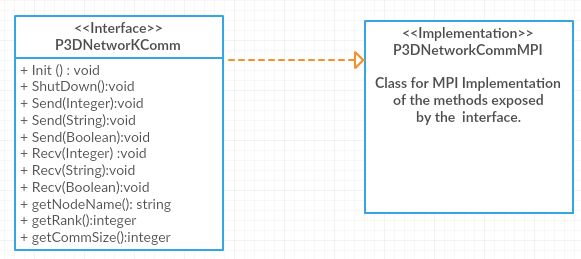
\includegraphics[scale=0.75]{Interface.png}
\caption{Class Diagram for the Interface}
\label{fig:InterfaceDiagram}
\end{figure}


\subsection{How does MS-MPI work internally?}

MPI as mentioned in the earlier sections provides the methods which allow for communication via message passing in a point-to-point communication or collective communication paradigm. MPI specifies a standard on what a message passing interface is supposed to do and not how it is done. The part of how it is done is decided by the implementation. The implementation can provide MPI methods using different underlying protocols and performance of the communication depends on the implementation, the underlying network and type of data communicated. MPI is message oriented protocol meaning that data is sent in distinct packets which are assembled at the receiver whereas a stream oriented protocol will have data sent byte-by-byte i.e. stream of bytes.The size of the data sent determines the way in which the message is sent or received. The underlying message protocol can be {\lq}eager{\rq} or {\lq}rendezvous{\rq} protocol\newline 

\textbf{Eager Message Passing Protocol}- The responsibility of storing the message is done at the receiver's end if no matching receive has been posted by the receiver. The sending process sends the message which is received by the receiving process if the matching receive has been already posted other wise the message is buffered by the receiving process. The sending process sends the message irrespective of whether the receive has been posted or not. It is allows for easy implementation of MPI\_Send and better performance as the send call does not need to block to get an acknowledgment from the receive operation. The problem is that this solution is not scalable and may lead to memory exhaustion if there are large number of messages which need to be buffered at the receiver. Another problem is the extra copy of the buffered message is required at the receiver from the buffered space i.e. the buffer allocated in the kernel space to the receiver's buffer i.e. the buffer allocated  in the receiver process's address space. This also leads to investing CPU cycles for the extra copy to be made.       

\textbf{Rendezvous Message Passing Protocol}- This protocol can be used on top of the eager protocol i.e. when the buffering limit has been reached. There is no underlying assumption made by the sending process that the receiver can allocate the memory and hence need to first signal the receiver process about the incoming message. This signaling is called as {\lq}handshake{\rq}. The format of the message for MPI was introduced in the  section \ref{MSMPI-API}. The Figure \ref{fig:MessageFormat} shows the message format specified by MPI standard \cite{mpiMsgForm}. During the handshake the following actions are performed in the specified order: 

\begin{enumerate}
\item The receiver process first receives the envelope of the message to be sent from the sender.
\item The received envelope is stored by the receiver process if there is no buffer space. 
\item As the buffer space becomes available, receiver process sends an acknowledgment to the sender, indicating that it can receive the message.
\item The sender after receiving the acknowledgment from the receiver, sends the actual payload. 
\item The receiver then receives the message. 
\end{enumerate}   

The protocols fixes the buffer exhaustion issue by not overwhelming the receiver's buffer by actual data rather the receiver needs to just store the envelope of the message which is relatively smaller in size. Therefore makes the receiver process more robust as the receiver does not hang because of buffer overflow. As the messages are received after the acknowledgment by the sender, CPU cycles are saved as the data can directly be copied to the buffer allocated in process's address space. The problem with this protocol is extra messages exchanged during the handshake. 

\begin{figure}[ht!]
\centering
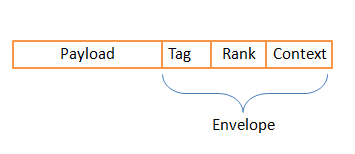
\includegraphics[scale=0.75]{MessageFormat.png}
\caption{Format of MPI Message}
\label{fig:MessageFormat}
\end{figure}

The receive event of a message can either be notified through an interrupt or the receiving process can poll at regular intervals to check if a message has arrived \cite{mpirel}. The interrupt technique works better when the send/receives are asynchronous i.e. they are non-blocking where as polling works well in case of synchronous send/receives i.e. they are blocking. In the polling mode,the receiver process busy waits using the CPU and queries the hardware frequently and manages the messaging by bypassing the OS where as in interrupt mode, the receiving process interacts with the OS which might decide to suspend the process while it is waiting for the message. As the time wasted in the context switch can be significant if the receive event is frequently done as well as OS involvement is generally costly, for better performance reasons the polling method is used by the implementations of MPI specification. \newline

MPI can use TCP/IP as the underlying protocol for message passing in a cluster connected via Infiniband i.e. TCP/IP over Infiniband (IPoIB) or it can use lower level protocols like the OpenFabric protocol or Qlogic Performance Scaled Messaging Protocol or it could as simple as TCP/IP over Ethernet. Microsoft's implementation of MPI-2 specification varies from others such that it uses mechanisms by which the use of TCP/IP can be bypassed. MS-MPI uses Microsoft WinSock Direct Protocol for compatibility over different kinds of Ethernet interconnect and CPU efficiency. The WinSock direct protocol \cite{SDP} uses remote direct memory access i.e. RDMA and thereby bypasses TCP/IP stack as it goes directly to the network interface card allowing for high-speed communication of data. When the TCP/IP stack is bypassed, the overhead occurred due to use of extra CPU cycles and memory bandwidth could be avoided. Winsock Direct Protocol reduces the library overhead and application distribution can scale better even over traditional interconnect networks. Figure \ref{fig:WinsockProto} depicts how the WinSock protocol works \cite{msmpiWinSoc}. \newline

\begin{figure}[ht!]
\centering
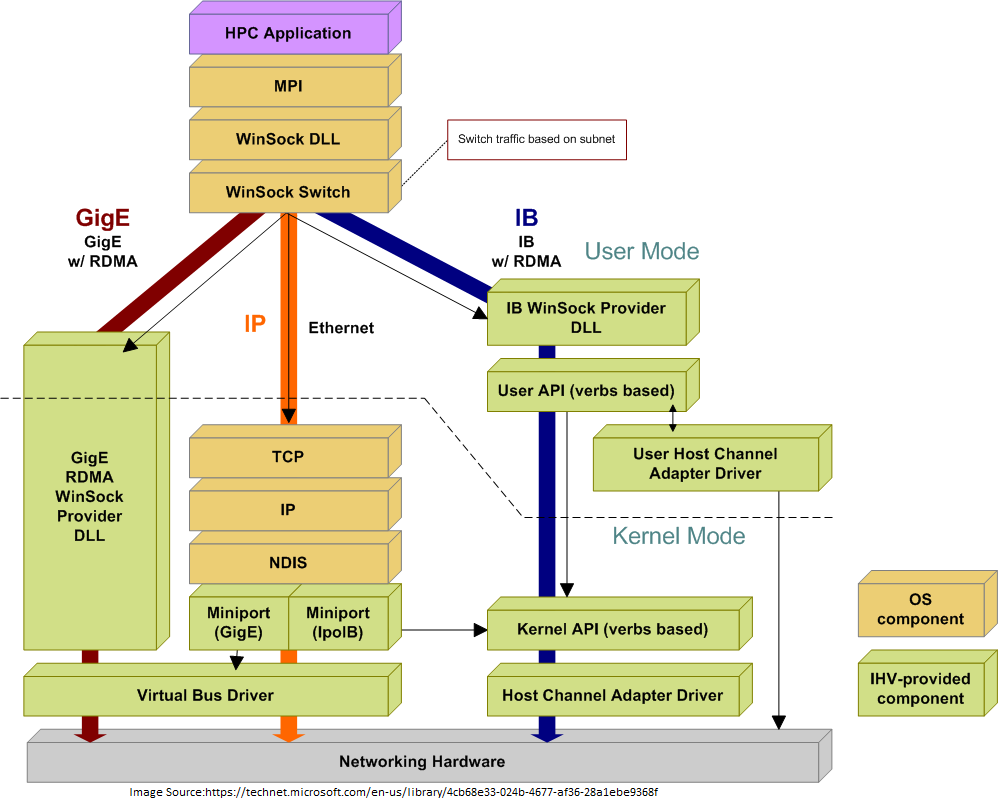
\includegraphics[scale=0.85]{WinSockProtocol.png}
\caption{WinSocket Direct Protocol Behavior}
\label{fig:WinsockProto}
\end{figure}
   
\section{Comparison of MPI to traditional socket programming}

MPI is designed to allow communication amongst HPC (high performance cluster) and preferred choice of programmers over traditional socket programming \cite{mpivssock}. The goal of programming applications to run on HPC is to perform huge and complex computation in a distributed manner if possible. To achieve this goal, programs which perform splitting of huge tasks into smaller sub-tasks and accumulation of partial results to generate final output are written. The logic to perform splitting of tasks, accumulation of results, synchronization and communication if needed among the cluster nodes requires significant programming effort and leads to complicated code. So, it is justified that the developers use libraries which abstract from the underlying complexities of communication but allow to write simple, clean and understandable code. MS-MPI is one such implementation of MPI-2 specification which not only provides decent performance but also lets developers not be bothered about managing the IP addresses, sockets/connection - opening and closing them, and other idiosyncrasies of the underlying network. Simple MPI\_SEND and MPI\_RECV calls do the magic necessary for successful communication. MPI allows to use customized proprietary networks leading to high-throughput and low latency communication. These networks provide abstractions which might not be suitable for socket programming and in-turn lead to lower performance of the application when sockets are used. \newline          

The problem with MPI-2 specification based implementation is lack of robustness when the communication fails amongst the network. There is no standardization of error management and reporting which leads to vague error messages being shown in an event of failure. This is where socket programming might win against MPI as level of robustness provided is pretty standard. Another issue with MS-MPI is that the spawning of the processes and group management is done when the application is launched and dynamic scaling up/down of cluster resources cannot be done at run-time. The cases where the number of sub-tasks are lowers than the configured cluster size needs to be handled by the implementation. So, when the number of print object files in the main configuration is less than the number slave nodes in the cluster, the master needs to drop some of the slaves from the cluster and only wait on {\lq} working nodes{\rq} for partial output. 
	
\section{External Libraries}
\section{Debugging}
\section{Project Management}